\section{Aufgabe 10}

In dieser Aufgabe sollte die Funktion propagate() für ein Teilchen mit
Mehrfachstreuung in 2D implementiert werden.

Zuerst wird für das Teilchen die Absorptionsdistanz bestimmt.
Diese folgt einer Exponentialverteilung mit der mittleren Reichweite $L_{absorption} = 150$ Einheiten.
Die Bestimmung der Absorptionsdistanz des Teilchens erfolgt dann einfach mit der auf dem letzten Blatt
implementierten Methode zur Erzeugung exponentialverteilter Zufallszahlen mit der
der Funktion propagate() übergebenen random\_state Instanz.

Anschließend streut das Teilchen immer wieder, bis es die Absorptionsdistanz erreicht hat.
Die Streudistanzen folgen dabei wieder einer Exponentialverteilung mit mittlerer Reichweite
$L_{scattering} = 10$ Einheiten. 

Dies wird durch eine while-Schleife gewährleistet, die solange TRUE ist, bis die
addierten Streudistanzen die Absorptionsdistanz überschreiten.

In jedem Schritt in dieser Schleife wird die Position und die Richtung des Teilchens aktualisiert.
Die Position ändert sich dabei immer um den Betrag der Streudistanz in Richtung
des über die AngleDistribution() berechneten neuen Winkels
\begin{equation*}
    \Psi_{new} = \Psi_{old} + \Delta\Psi \;.
\end{equation*}
In jedem dieser Schritte wird auch ein neuer Eintrag in der Tupelliste energy\_depositions gemacht,
welche die Form ($x$, $y$, $E_{dep}$, $\Psi$) hat.
Dieser Prozess wird wiederholt, bis das Teilchen absorbiert wurde.

Der erste Eintrag ist dabei vom Teilchen abhängig, meistens aber ($0$, $0$, $0$, $0$).
Das Teilchen deponiert erst im letzten Schritt, wenn es die Absorptionsdistanz erreicht hat, alle seine Energie.

In den Plots in Abbildung \ref{fig:mcmultiplescattering} erkennt man im Plot oben links,
wie das Teilchen streut und dabei seine Richtung ändert und dabei zufällig weit streut.
In den unteren beiden Plots ist zu erkennen, dass unsere Streu- und unsere Absorptionsdistanzen einer 
Exponentialverteilung folgen.

\begin{figure}
    \centering
    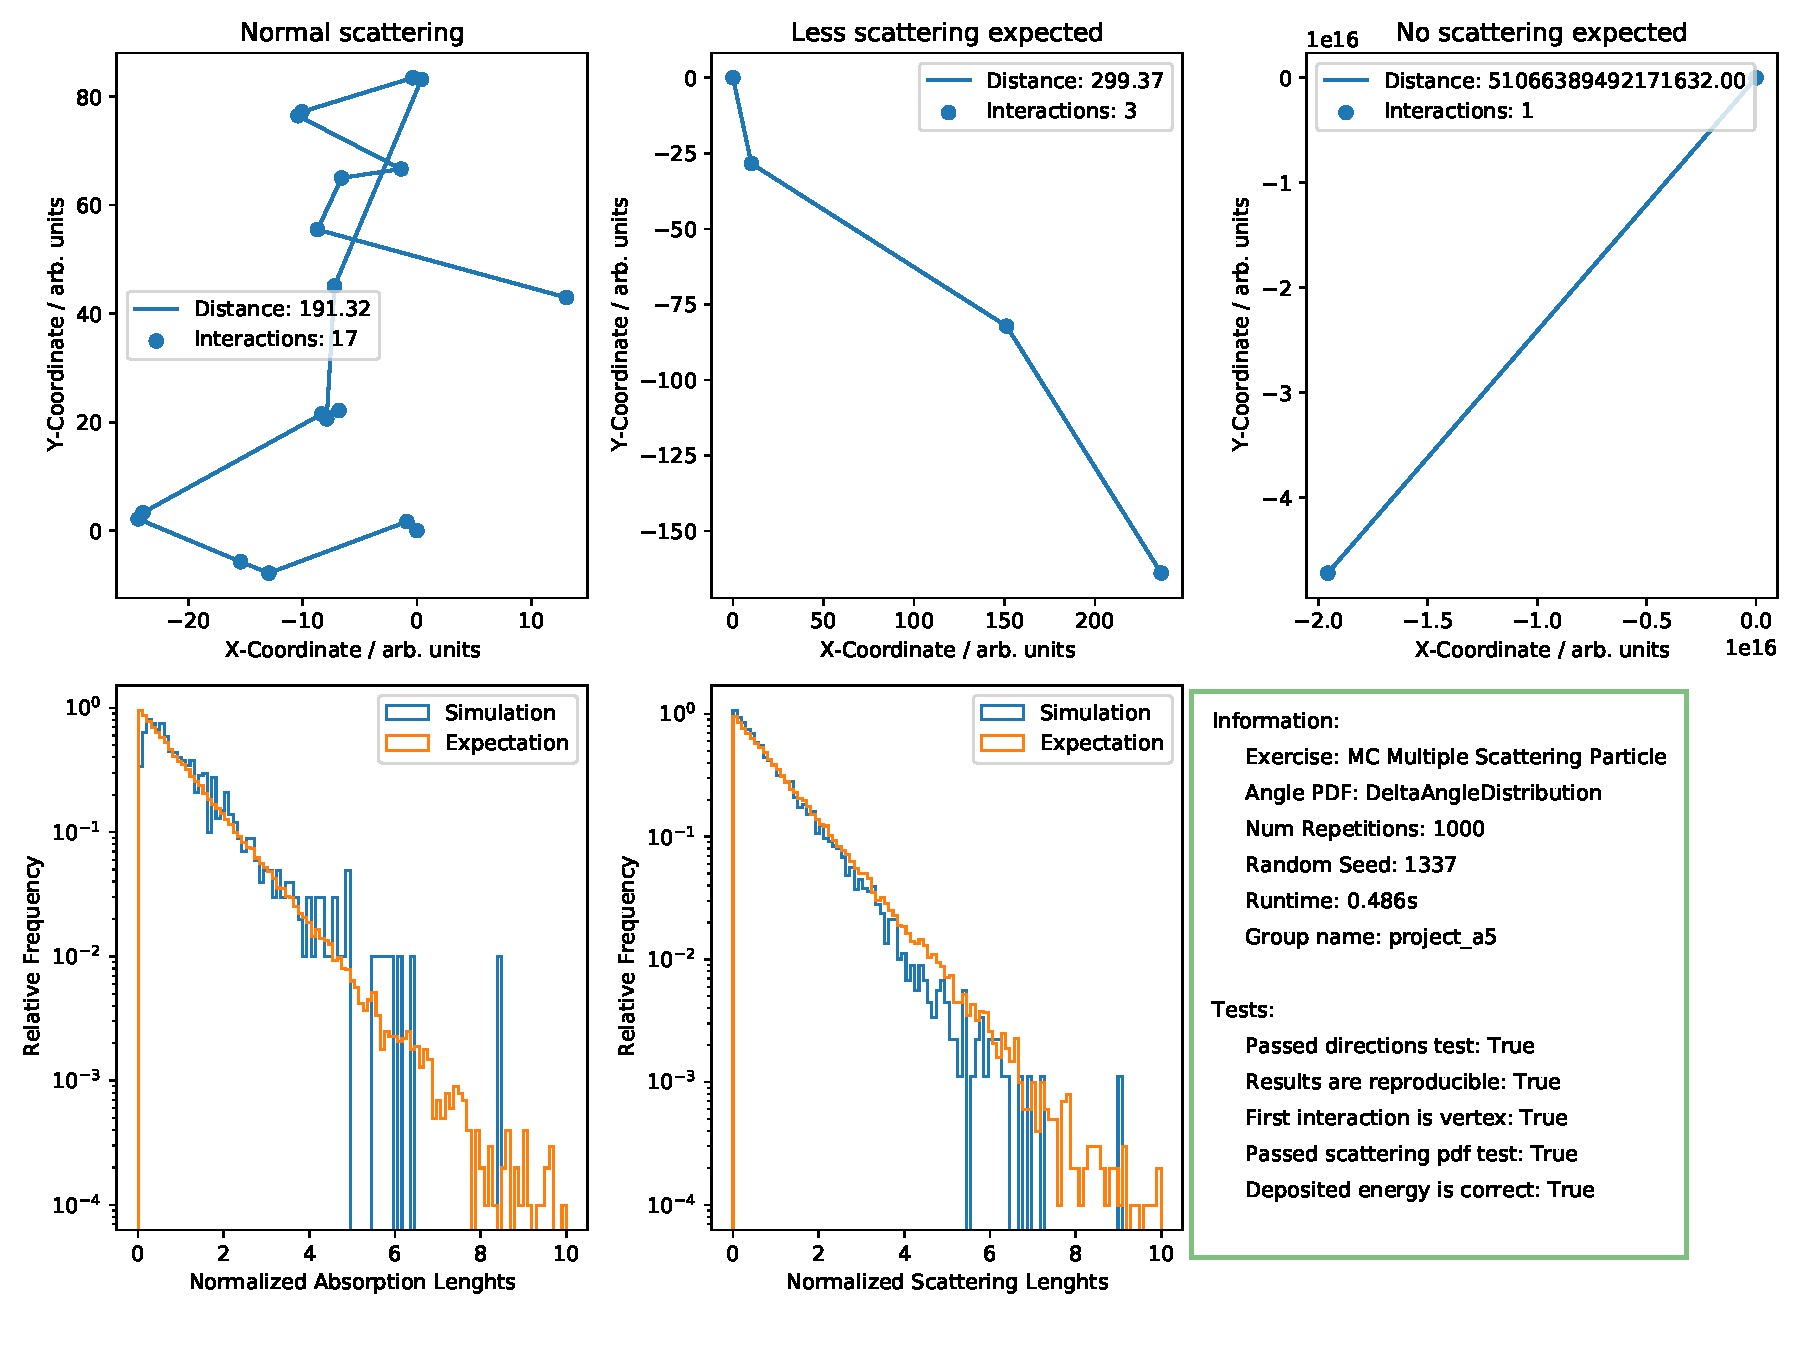
\includegraphics[width=\textwidth]{Aufgabe10/exercise_mc_multiple_scattering.pdf}
    \caption{Übersicht der Plots.}
    \label{fig:mcmultiplescattering}
\end{figure}